% Part: sets-functions-relations
% Chapter: infinite
% Section: hilberts-hotel
%
\documentclass[../../../include/open-logic-section]{subfiles}

\begin{document}

\olfileid[pt]{sfr}{infinite}{hilbert}
\olsection{Hotel de Hilbert}

O conjunto dos números naturais é obviamente infinito. Logo, se não
quisermos \emph{valer-nos} dos números naturais, o nosso primeiro
passo é caracterizar um conjunto infinito em termos que não
exijam mencionar os próprios números naturais. Eis uma abordagem
agradável, apresentada por Hilbert numa conferência de 1924. Ele nos pede
que imaginemos
\begin{quote}
[\ldots] um hotel com um número finito de quartos. Todos esses quartos
devem estar ocupados por exatamente um hóspede. Se os hóspedes trocam
de quarto de algum modo, [mas] de tal forma que cada quarto continua a
conter no máximo uma pessoa, então nenhum quarto ficará livre, e o dono
do hotel não pode, deste modo, criar um novo lugar para um hóspede que
acaba de chegar [\ldots
\textparagraph \ldots]

Agora estipulamos que o hotel tem infinitos quartos numerados
$1$, $2$, $3$, $4$, $5$, \dots, cada um ocupado por exatamente um
hóspede. Logo que chega um novo hóspede, o dono só precisa de mudar
cada um dos hóspedes antigos para o quarto associado ao número imediatamente
superior, e o quarto~$1$ ficará livre para o recém-chegado.
	\begin{center}
		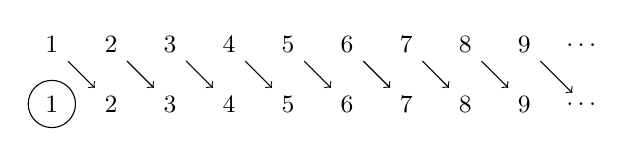
\begin{tikzpicture}[scale = .75]
		\foreach \x in {1, 2, 3, 4, 5, 6, 7, 8, 9}
		{
			\node (\x a) at (\x, 1) {\small{\x}};
			\node (\x b) at (\x, 2) {\small{\x}};
		}
		\node (dotsa) at (10, 1) {\small{\ldots}};
		\node (dotsb) at (10, 2) {\small{\ldots}};
		\draw[->] (1b)--(2a);
		\draw[->] (2b)--(3a);
		\draw[->] (3b)--(4a);
		\draw[->] (4b)--(5a);
		\draw[->] (5b)--(6a);
		\draw[->] (6b)--(7a);
		\draw[->] (7b)--(8a);
		\draw[->] (8b)--(9a);
		\draw[->] (9b)--(dotsa);
		\draw (1,1) circle (.4);
		\end{tikzpicture}
	\end{center}
	(publicado em \citealt[730]{EwaldSieg2013}; a nossa tradução)
\end{quote}
O ponto crucial é que o Hotel de Hilbert tem infinitos quartos;
e podemos tomar a sua explicação como definição do que significa dizer
isto. De fato, foi esta a abordagem de Dedekind (apresentada aqui, claro,
com enorme anacronismo; a definição de Dedekind é de
\citeyear{Dedekind1888}):

\begin{defn}\ollabel{defn:DedekindInfinite}
Um conjunto $A$ é \emph{infinito de Dedekind} sse existe !!a{injection}
de~$A$ para um subconjunto próprio de~$A$. Isto é, existe algum $o \in A$
e !!a{injection} $f \colon A \to A$ tal que $o \notin \ran{f}$.
\end{defn}

\end{document}
